\documentclass[review]{elsarticle}

\usepackage{lineno,hyperref}
\modulolinenumbers[5]

\journal{Journal of \LaTeX\ Templates}

%%%%%%%%%%%%%%%%%%%%%%%
%% Elsevier bibliography styles
%%%%%%%%%%%%%%%%%%%%%%%
%% To change the style, put a % in front of the second line of the current style and
%% remove the % from the second line of the style you would like to use.
%%%%%%%%%%%%%%%%%%%%%%%

%% Numbered
%\bibliographystyle{model1-num-names}

%% Numbered without titles
%\bibliographystyle{model1a-num-names}

%% Harvard
%\bibliographystyle{model2-names.bst}\biboptions{authoryear}

%% Vancouver numbered
%\usepackage{numcompress}\bibliographystyle{model3-num-names}

%% Vancouver name/year
%\usepackage{numcompress}\bibliographystyle{model4-names}\biboptions{authoryear}

%% APA style
\bibliographystyle{model5-names}\biboptions{authoryear}

%% AMA style
%\usepackage{numcompress}\bibliographystyle{model6-num-names}

%% `Elsevier LaTeX' style
%\bibliographystyle{elsarticle-num}
%%%%%%%%%%%%%%%%%%%%%%%

% ---------------------
% Pacotes OBRIGATÓRIOS
% ---------------------
%\usepackage{lmodern}				% Usa a fonte Latin Modern			
\usepackage[T1]{fontenc}			% Selecao de codigos de fonte.
\usepackage[utf8]{inputenc}		% Codificacao do documento (conversão automática dos acentos)
%\usepackage{lastpage}			% Usado pela Ficha catalográfica
%\usepackage{indentfirst}			% Indenta o primeiro parágrafo de cada seção.
\usepackage{color}			     	% Controle das cores
\usepackage{graphicx}	         % Inclusão de gráficos
\usepackage{epsfig,subfig}		% Inclusão de figuras
\usepackage{microtype} 			% Melhorias de justificação
% ---------------------

% ---------------------
% Pacotes ADICIONAIS
% ---------------------
\usepackage{lipsum}						% Geração de dummy text
\usepackage{amsmath,amssymb,mathrsfs, amsthm}	% Comandos matemáticos avançados 
\usepackage{setspace}  					% Para permitir espaçamento simples, 1 1/2 e duplo
\usepackage{verbatim}					% Para poder usar o ambiente "comment"
\usepackage{tabularx} 					% Para poder ter tabelas com colunas de largura auto-ajustável
\usepackage{afterpage} 					% Para executar um comando depois do fim da página corrente
\usepackage{url} 						% Para formatar URLs (endereços da Web)
\usepackage{todonotes}  		% Lista de afazeres To-dos
\usepackage{enumitem}					% Fazer enumerações por letras ou números nos itens

% Configura o ambiente de teoremas, definições etc.

\theoremstyle{definition} 
\newtheorem{teor}{Teorema}%[section]
\newtheorem{defi}[teor]{Definição}
\newtheorem{lema}[teor]{Lema}
\newtheorem{supo}[teor]{Suposição}
\newtheorem{exemplo}[teor]{Exemplo}
\newtheorem{prop}[teor]{Proposição}


\begin{document}

\begin{frontmatter}

\title{Medida condicional de \emph{Expected Shortfall} nos mercados latinoamericanos através da teoria do valor extremo\tnoteref{mytitlenote}}
\tnotetext[mytitlenote]{Fully documented templates are available in the elsarticle package on \href{http://www.ctan.org/tex-archive/macros/latex/contrib/elsarticle}{CTAN}.}

%% Group authors per affiliation:
%\author{Rafael Felipe Bressan\fnref{myfootnote}\corref{correspondente}}
%\address{Avenida Madre Benvenuta, 2007 - Santa Mônica Florianópolis - SC 88035-901}
%\fntext[myfootnote]{Depto. de Economia/Esag/UDESC}

%% or include affiliations in footnotes:
\author[mymainaddress,mysecondaryaddress]{Elsevier Inc}
\ead[url]{www.elsevier.com}

\author[mymainaddress]{Rafael Felipe Bressan\corref{mycorrespondingauthor}\fnref{myfootnote}}
\cortext[mycorrespondingauthor]{Corresponding author}
\ead{rafael.bressan@edu.udesc.br}
\fntext[myfootnote]{Depto. de Economia/Esag/UDESC}

\address[mymainaddress]{Avenida Madre Benvenuta, 2007 - Santa Mônica Florianópolis - SC 88035-901}
\address[mysecondaryaddress]{360 Park Avenue South, New York}

\begin{abstract}
This template helps you to create a properly formatted \LaTeX\ manuscript.
\end{abstract}

\begin{keyword}
\texttt{elsarticle.cls}\sep \LaTeX\sep Elsevier \sep template
\MSC[2010] 00-01\sep  99-00
\end{keyword}

\end{frontmatter}

\linenumbers

\section{Introdução}

\paragraph{A medição do risco de mercado} ao qual os portfólios dos investidores está sujeito é objeto de devoção de esforços tanto por parte das instituições e investidores em geral como por parte dos reguladores. Instituições financeiras em todo o mundo, de acordo com suas regulações locais e com os princípios de Basileia (\emph{Basel Comittee on Banking Supervision} - BCBS do Banco de Compensações Internacionais - BIS\footnote{http://www.bis.org/bcbs/index.htm?m=3\%7C14}) para aquelas que o seguem (o Brasil é um desses países)  são obrigadas a reservar uma parcela de seu capital como provisionamento contra flutuações adversas do mercado em seus portfólios de investimento.

Uma importante característica das séries de retornos financeiros é sua alta volatilidade, não constante e tampouco seguindo a distribuição Normal. Assim, eventos extremos, e neste caso estamos interessados em perdas de grande magnitude, acontecem com uma frequência alta demais para serem descartadas como apenas \emph{outliers}, e portanto passaram a atrair a atenção dos participantes do mercado, entre eles os investidores e também os reguladores. Estas observações induziram uma gama enorme de estudos, práticos e teóricos, voltados a explicar o comportamento dos retornos de séries financeiras e modelar de forma adequada as caudas da distribuição destes retornos. Não somente estes estudos são de grande relevância para o gerenciamento de risco nas instituições financeiras, como também são obrigatórios segundo o acordo de Basileia, uma vez que este requer o cálculo do Valor em Risco - VaR, para então a instituição poder projetar o seu nível requerido de capital. 

De acordo com os princípios de Basileia III, \cite{BCBS2011, BCBS2013, BCBS2014}, as instituições financeiras supervisionadas pelos Bancos Centrais devem manter \emph{buffers} de capital contra riscos de mercado, crédito, liquidez, entre outros. Dentro dos riscos de mercado, as duas formas mais usuais de fazer a quantificação destes são os métodos de Valor em Risco - VaR e o \emph{Expected Shortfall} - ES. Este último relacionado ao primeiro, sendo definido como o valor esperado das perdas que excedem o valor VaR calculado para um determinado intervalo de confiança.
\todo{Percentuais de VaR por Basileia}
\todo{Existem penalidades regulatórias para as IF em que seu modelo VaR permite um número maior de perdas do que seria estimado pelo modelo. Verificar onde nos princípios de Basileia}

VaR é um quantil $\alpha$ da distribuição de perdas de um ativo ou portfólio em um determinado período de tempo, ao passo que ES é o valor esperado das perdas que excedem VaR, para um mesmo intervalo de confiança $\alpha$ e período.

O método VaR para cálculo de risco de mercado ao qual um portfólio está sujeito foi primeiramente introduzido através de \cite{RiskMetrics1995}, uma metodologia adotada pelo banco J. P. Morgan. Vem desde então sendo amplamente adotado pela indústria financeira e largamente estudado pela academia. Inúmeras variantes do modelo foram propostas e continuam sendo utilizadas com o passar dos anos. Para o cálculo do VaR é necessária uma suposição acerca da distribuição dos retornos, e por conseguinte do comportamento da cauda desta.

As variações na metodologia original de estimação do VaR surgem principalmente em função de críticas a abordagem proposta, a qual inclui a suposição de retornos independentes e igualmente distribuídos (\emph{iid}), covariâncias constantes entre os ativos de um portfólio e a distribuição normal dos retornos.

Uma das últimas fortes críticas a medida do VaR, e que deu origem a outra métrica conhecida como \emph{Expected Shotfall}, ou simplesmente ES, veio de dois artigos \cite{Artzner1997} e \cite{Artzner1999}. Primeiramente foram introduzidas quatro propriedades cunhadas através de axiomas, as quais medidas coerentes de risco deveriam possuir, sendo elas: 

\begin{itemize}
	\item invariância a translação;
	\item sub-aditividade;
	\item homogeneidade positiva, e;
	\item monotonicidade.
\end{itemize}

VaR especificamente não possui a propriedade da sub-aditividade para alguns casos. Para contornar este fato, \cite{Acerbi2002} propõe o \emph{Expected Shortfall} e comprovam que este é uma medida coerente de risco. Além de ser coerente, o ES possui uma segunda vantagem com relação ao VaR, considerando que o ES nos informa uma medida de tendência central do tamanho das perdas que excedem o valor do quantil VaR. Ou seja, o VaR nos informa apenas que uma proporção $\alpha$ das perdas serão menor que a medida, mas nada nos informa se esta perda extraordinária de fato ocorrer. Mesmo sendo criticado e demonstradamente uma medida não coerente de risco, o VaR continua a ser amplamente utilizado, mesmo que agora em conjunto com o ES. 

Mais recentemente o Comitê de Supervisão Bancária de Basileia tem se proposto a adotar o \emph{Expected Shortfall} como medida de risco de mercado. \cite{BCBS2013a}. O Comitê cita a grande importância da escolha da medida de risco e sua calibração, e portanto estas são relevantes para as decisões de política do Banco. Entre as dificuldades encontradas pelo VaR estão mais notadamente sua inabilidade em estimar o "risco de cauda" da distribuição de perdas, uma vez que VaR não leva em conta a distribuição das perdas acima do valor de corte.

Desta forma, foi decidido que o ES seria a medida de risco favorita para a abordagem pelo banco chamada de modelos internos. Ou seja, os bancos supervisionados devem utilizar o ES para o cálculo do risco de mercado a que estão sujeitos em seus modelos internos. O comitê também se decidiu por um intervalo de confiança de 97,5\% para o ES, em contraposição a 99\% para o VaR. O comitê espera que esta abordagem para o cálculo da medida de risco de mercado trará benefícios se comparada a antiga abordagem pelo Var, entre elas um modelo com resultados mais estáveis e menor sensibilidade a observações extremas (\emph{outliers}).

\paragraph{Teoria do valor extremo} EVT da sigla em inglês, é um ramo da estatística que lida diretamente com eventos raros, extremos. Seu objetivo é modelar eventos que se distanciam muito da mediana de uma distribuição. Justamente por esta característica, a EVT está sendo utilizada para modelar riscos que possuem distribuição com caudas longas, um dos fatos estilizados que apresentamos sobre retornos de ativos financeiros.

Ao utilizarmos a EVT, e mais especificamente o método conhecido como \emph{peaks over treshold} – POT, estamos interessados em modelar apenas a parte da cauda da distribuição das perdas de um ativo financeiro maiores que um determinado valor de limiar \emph{u}. É da modelagem desta cauda, portanto, que faremos as estimativas de risco $VaR_\alpha$ e $ES_\alpha$.

\section{O método \emph{peaks over treshold}}

Consideremos uma amostra de uma variável aleatória (v.a.) cujas observações sejam independentes e igualmente distribuídas (i.i.d.), $L_i,i\in \mathbb{N}$, que represente as perdas financeiras de um determinado ativo.

A EVT está interessada em investigar o comportamento da distribuição dos máximos desta v.a. dados por $M_n = \max (L_1, \ldots , L_n)$ para vários valores de $n$ e a medida que $n\rightarrow \infty$. A sequência $M_n$ é chamada de máximos em bloco e é possível demonstrar que a única distribuição para a qual $M_n$ converge com $n\rightarrow \infty$ é a distribuição de valores extremos generalizada (GEV, da sigla em inglês).

%Para tanto, é necessário normalizarmos esta sequência de máximos de forma que sua distribuição seja convergente para uma distribuição $H(x)$ não-degenerada. Seja $F(x)$ a distribuição original de uma variável aleatória \emph{iid}, é possível normalizar seus máximos em bloco através da relação $M_n^*=(M_n-d_n)/c_n$ de forma que:
%
%\begin{equation}
%\label{eq:H}
%\lim_{n \rightarrow \infty} P\left(\frac{M_n-d_n}{c_n} \leq x \right) 
%= \lim_{n \rightarrow \infty} F^n(c_nx + d_n)
%= H(x)
%\end{equation}

%Em outras palavras, para determinadas sequências $c_n$ e $d_n$ a serem escolhidas, existe uma distribuição de $H(x)$ não-degenerada a qual representa a distribuição dos máximos em bloco de $F(x)$.
%
%A potenciação de $F$ em $n$ deriva diretamente da suposição que a variável aleatória é iid, enquanto que a transformação de $x \rightarrow c_n x+d_n$ é a normalização dos máximos em bloco.

\begin{defi}[MDA] \label{defi:MDA}
	Domínio de máxima atração, se a equação \eqref{eq:H} é válida para uma $H$ não-degenerada, então se diz que $F \in MDA(H)$, $F$ pertence ao domínio de máxima atração de $H$.
\end{defi}

\begin{teor}[Fisher-Tippett, Gnedenko] \label{teor:fisher-tippett}
	Se $F \in MDA(H)$ para alguma $H$ não-degenerada, então $H$ deve ser uma distribuição do tipo de valores extremos generalizada – GEV.
\end{teor}
O teorema \ref{teor:fisher-tippett} foi estabelecido através de três artigos, \cite{Fisher1928}, \cite{Gnedenko1941, Gnedenko1943}.

\begin{defi}[GEV] \label{defi:GEV}
	Distribuição de valores extremos generalizada, é definida por sua p.d.f (função densidade de probabilidades) a qual é dada por:
\end{defi}

\begin{equation}
\label{eq:GEV}
H_\xi(x) = 
\begin{cases}
exp(-(1+\xi x)^{-\frac{1}{\xi}}), & \xi \neq 0,\\
exp(-e^{-x}), & \xi = 0,\\
\end{cases}
\end{equation}

O parâmetro $\xi$ é conhecido como o parâmetro de forma da distribuição e dependendo deste valor teremos diferentes tipos de distribuição (casos particulares da GEV). Quando $\xi=0$ a distribuição resultante é uma Gumbel, quando  $\xi>0$ uma Fréchet surge, e por fim quando $\xi<0$ temos uma Weibull.

Para as aplicações financeiras não necessitamos calcular a qual $MDA$ pertencem nossas distribuições contínuas, bastando saber que basicamente todas as distribuições de utilidade prática estão contidas em $MDA(H_\xi)$ para algum valor de $\xi$ \cite[p. ~139]{McNeil2015}.

\subsection{Excessos acima de um limiar}
\label{sec:excess}

O método conhecido como POT, para calcular a função de distribuição dos valores que excedem um determinado limiar de um conjunto de dados vem sendo empregado no mundo financeiro para ajustar as caudas das distribuições de retornos, ou perdas, dos ativos. Este método é preferido a teoria clássica de valores extremos (e.g. máximos em bloco), pois, desperdiça uma quantidade menor de dados da série original. Qualquer valor que exceda o limiar pré-determinado é considerado na distribuição dos excessos. Esta distribuição dos valores da série que estão acima de um determinado limiar \emph{u} é definida como:

\begin{defi}[Distribuição dos excessos] \label{defi:excess}
	Seja \emph{X} uma variável aleatória com função de distribuição \emph{F}. A distribuição dos excessos sobre um limiar \emph{u} tem a seguinte função de distribuição:
\end{defi}

\begin{equation}
\label{eq:excessdist}
F_u(x)=P(X-u \leq x | X > u)=\frac{F(x+u)-F(u)}{1-F(u)}
\end{equation}
para $0 \leq x < x_F-u$, onde $x_F \leq \infty$ é o limite direito da distribuição \emph{F}.

Uma importante distribuição que surge na modelagem dos excessos sobre um limiar é a distribuição gereralizada de pareto – GPD, que segue.

\begin{defi}[GPD] \label{defi:GPD}
	Distribuição de Pareto Generalizada é definida por sua função de distribuição:
\end{defi}

\begin{equation}
\label{eq:GPD}
G_{\xi,\beta(u)}(X) = 
\begin{cases}
1- \left(1+ \frac{\xi x}{\beta(u)} \right)^{-\frac{1}{\xi}}, & \xi \neq 0,\\
1-exp\left(-\frac{x}{\beta(u)}\right), & \xi = 0,\\
\end{cases}
\end{equation}
onde $\beta > 0$, e $x\geq 0$ quando $\xi  \geq 0$ ou $0 \leq x \leq -\beta / \xi$ quando $\xi < 0$.

Os parâmetros $\xi$ e $\beta$ são conhecidos respectivamente como parâmetros de forma e escala da distribuição. 

A distribuição generalizada de Pareto tem papel fundamental na teoria de valor extremo em função do teorema de Pickands-Balkema-de Haan (\cite{Pickands1975} e \cite{Balkema1974}) conforme abaixo:

\begin{teor}[Pickands-Balkema-de Haan]
	\label{teor:pickands}
	Pode ser encontrada uma função $\beta(u)$ tal que:
	\begin{equation*}
	\lim\limits_{u \rightarrow x_F} \; \sup\limits_{0\leq x <x_F - u} |F_u(x)-G_{\xi, \beta(u)}(x)| = 0 
	\end{equation*}
	se e somente se $F\in MDA(H_\xi)$ para $\xi \in \mathbb{R}$.
\end{teor}

O que este teorema nos diz é que para distribuições as quais os máximos em bloco normalizados convergem para uma GEV (na forma da equação \eqref{eq:GEV}), então a distribuição dos excessos acima de um limiar destas mesmas distribuições convergem para uma GPD, dado um valor de limiar \emph{u} adequado. Como para fins práticos basicamente todas as distribuições contínuas de fato estão no $MDA(H_\xi)$ para algum valor de $\xi$, temos que a GPD é a distribuição a ser escolhida para modelar excessos acima de um limiar.

Ao fazermos a suposição que a distribuição dos excessos \emph{é igual} a uma GPD, podemos então a partir dos dados de perdas estimar os parâmetros de forma e escala e portanto, modelar a cauda direita da nossa distribuição de perdas de forma parametrizada. Esta é uma suposição, uma vez que a distribuição dos excessos não segue exatamente uma GPD, mas apenas tende a esta distribuição dado um limiar \emph{u} alto e uma amostra de dados grande o suficiente.

Dada a parametrização de uma GPD, é interessante sabermos o valor esperado desta distribuição, uma vez que esta medida de valor central nos fornece importante informação sobre a quantidade de risco que estamos buscando medir, assim como a informação de que a própria distribuição foi ajustada aos dados de forma satisfatória, como será demonstrado adiante.

\begin{defi}[função média dos excessos]
	\label{defi:meanexcess}
	A função média dos execessos de uma variável aleatória \emph{X} com média finita é dada por:
\end{defi}

\begin{equation}
\label{eq:meanexcess}
e(u)=E\left(X-u | X > u\right)
\end{equation}

Ou seja, a equação \eqref{eq:meanexcess} representa o valor esperado da função de distribuição dos excessos dada pela Definição \ref{defi:excess}. Ela representa a média de $F_u$ como uma função do limiar \emph{u}. Esta função por vezes também é conhecida como função média de vida residual (\emph{mean residual life function}), sendo encontrada esta denominação em alguns pacotes de \emph{software} estatísticos.

Para uma variável distribuída na forma de uma GPD, o parâmetro de escala é uma função linear em \emph{u} dado por $\beta(u)=\beta + \xi u$, \cite[Teorema 3.4.13(e)]{Embrechts1997}. Utilizando-se deste fato e da equação \eqref{eq:meanGPD} chegamos ao cálculo da função média dos excessos para uma GPD, dada por:

\begin{equation}
\label{eq:eu}
e(u)=\frac{\beta+\xi u}{1-\xi}
\end{equation}
onde $0 \leq u < \infty$ se $0 \leq \xi <1$ e $0 \leq u \leq -\beta / \xi$ se $\xi < 0$. É possível observar que de fato a função média dos excessos em uma GPD é linear em \emph{u}. Esta é uma característica importante de uma GPD e que nos auxilia a escolher um valor adequado do limiar \emph{u} de tal forma que a Suposição \ref{supo:excessdist} faça sentido.

%Assim, quando estamos analisando uma determinada distribuição de perdas \emph{F} e desejamos ajustar a cauda desta distribuição, ou seja, as perdas acima de um dado valor limiar \emph{u} a uma GPD $G_{\xi, \beta}(x)$ precisamos primeiramente determinar um valor adequado de \emph{u} de modo que a Suposição \ref{supo:excessdist} de que $F_u(x)\rightarrow G_{\xi, \beta}(x)$ seja válida. Um método frequentemente utilizado é o gráfico da função média dos excessos com relação a \emph{u}. Analisando este gráfico, escolhemos o menor valor de \emph{u} para o qual a partir deste ponto a relação $e(u) \text{ vs } u$ torna-se linear.
%
%Desejamos o menor valor de \emph{u} para o qual a relação é linear pois, mesmo o método POT implica em grande perda de dados da série temporal, já que apenas os valores acima deste limiar são utilizados para fazer a estimação dos parâmetros $\xi$ e $\beta$ da GPD. Portanto, existe um \emph{trade-off} na escolha do valor limiar \emph{u}, escolhendo um valor muito baixo termos uma boa quantidade de dados para estimar os parâmetros da GPD, mas a própria distribuição resultante não será GPD, uma vez que não estaremos trabalhando na região onde a relação $e(u) \text{ vs } u$ é linear. Por outro lado, um valor limiar muito alto nos impõe o custo de trabalhar com poucos dados para fazer a estimação dos parâmetros da distribuição e por conseguinte, os erros padrões dessas estimativas serão elevados.

\begin{lema} \label{lema:ev}
	Sob a Suposição \ref{supo:excessdist} segue que $F_v (x)=G_{\xi,\beta+\xi(v-u)} (x)$ para qualquer valor limiar $v \geq u$.
\end{lema}

Logo, a distribuição dos excessos sobre limiares mais altos que \emph{u}, também segue uma GPD com o mesmo parâmetro de forma $\xi$ e parâmetro de escala que cresce linearmente com este limiar mais alto \emph{v}. Se $\xi < 1$, a média desta nova GPD converge e é dada por:

\begin{equation}
\label{eq:ev}
e(v)=\frac{\beta+\xi(v-u)}{1-\xi}=\frac{\xi v}{1- \xi}+ \frac{\beta-\xi u}{1-\xi}
\end{equation}

Esta é a função média dos excessos sobre limiares mais altos, e está definida para $u \leq v < \infty$ se $0 \leq \xi < 1$ e, $u \leq v \leq u-\beta / \xi$ se $\xi < 0$.

Esta função é muito útil para calcularmos o $ES_\alpha$ (\emph{expected shortfall}), considerando que $VaR_\alpha$ nada mais é que um quantil superior ao limiar $u$ escolhido.

\section{Modelando caudas e medidas de risco associadas}
\label{sec:caudas}

Através da modelagem da cauda da distribuição \emph{F} de perdas por uma GPD, como feito na seção anterior, é possível calcularmos as medidas de riscos $VaR_\alpha \text{ e } ES_\alpha$ para esta distribuição de perdas em função dos parâmetros da GPD estimada e também fazendo uso da distribuição empírica de \emph{F}.

Sob a Suposição \ref{supo:excessdist} nós temos que a cauda da distribuição \emph{F}, $\bar{F}(x)$, para $x \geq u$ é dada por:

\begin{align}
\label{eq:Ftail}
\bar{F}(x) & = P(X>u)P(X>x|X>u) \nonumber \\
& = \bar{F}(u) P(X-u>x-u|X>u) \nonumber \\
& = \bar{F}(u)\bar{F}_u(x-u) \nonumber \\
& = \bar{F}(u)\left(1+\xi \frac{x-u}{\beta}\right)^{-1/\xi}
\end{align}

Da qual se soubéssemos exatamente a distribuição \emph{F} teríamos um modelo analítico para as probabilidades de perdas na cauda da distribuição. Aqui $x$ são os valores a serem observados das perdas, e portanto $x-u$ são as perdas em excesso ao limiar.

O que fizemos através da equação \eqref{eq:Ftail} foi efetivamente separar a distribuição \emph{F}, ou melhor, sua cauda, em duas partes. A primeira parte, para valores menores que \emph{u}, não foi modelado analiticamente e portanto utilizamos a distribuição empírica das perdas, aqui representada por sua cauda $\bar{F}(u)$, que nada mais é que o número observado de excessos de \emph{u} sobre o número total de observações da amostra.

A segunda parte é justamente a modelagem através de uma GPD com parâmetros $\xi \text{ e } \beta$ dado o limiar \emph{u}. Por esta modelagem paramétrica podemos conhecer as probabilidades de cauda para valores de \emph{x} maiores que \emph{u}.

O quantil $\alpha$ é a inversa da função distribuição e nos retorna o valor para o qual um percentual $\alpha$ de observações da amostra é menor ou igual. Assim sendo, $VaR_\alpha$ nada mais é que um quantil alto para o qual determinamos que $\alpha \%$ das perdas devem ser menores ou iguais a este valor.

Como a equação \eqref{eq:Ftail} fornece a probabilidade de cauda, então esta é igual a $1- \alpha$ para um valor de $\alpha  \geq F(u)$. Fazendo $\bar{F}(x)=1-\alpha$ na equação \eqref{eq:Ftail} o valor de \emph{x} representará $VaR_\alpha$ e nos basta manipular esta equação até isolarmos $VaR_\alpha$ como função de $\bar{F}(u), \alpha \text{ e dos parâmetros da GPD } \xi \text{ e } \beta$. Que nos garante a equação abaixo:

\begin{equation}
\label{eq:VaRGPD}
VaR_\alpha = q_\alpha(F) = u+\frac{\beta}{\xi}\left[ \left( \frac{1-\alpha}{\bar{F}(u)}\right)^{-\xi}-1 \right]
\end{equation}

A medida $ES_\alpha$ pode ser entendida como a média das perdas que excedem o valor dado por $VaR_\alpha$. Como o próprio $VaR_\alpha$ é um quantil acima do valor de limiar \emph{u}, $ES_\alpha$ é dado pelo valor do $VaR_\alpha$ somado a função média dos excessos dada pela equação \eqref{eq:ev} fazendo $v = VaR_\alpha$. Esta média é convergente para valores de $\xi < 1$ conforme já demonstrado. Ou seja, $ES_\alpha=VaR_\alpha + e(VaR_\alpha)$. A qual nos rende de forma mais geral:

\begin{equation}
\label{eq:ESGPD}
ES_\alpha = \frac{VaR_\alpha}{1-\xi}+\frac{\beta-\xi u}{1-\xi}
\end{equation}

Portanto, ambas medidas de risco $VaR_\alpha$ e $ES_\alpha$, para distribuições de perdas que tiveram suas caudas modeladas através de uma GPD da forma $G_{\xi, \beta(u)}$ com $\xi <1 \text{ e } \beta > 0$, podem ser calculadas respectivamente através das equações dadas em \eqref{eq:VaRGPD} e \eqref{eq:ESGPD}. As estimativas destas medidas de risco serão encontradas através das estimativas dos parâmetros da GPD, assim como do limiar utilizado e de uma medida empírica de $\bar{F}(u)$ que será o número de excessos verificados sobre o total de amostras. É claro que, ao adotarmos esta estimativa para $\bar{F}(u)$ estamos implicitamente supondo que o número de amostras na série de perdas é significativa, assim como o número de excessos verificados. Daí a importância de se utilizar um valor \emph{u} adequado, conforme explicitado na seção \ref{sec:excess}. \todo{Incluir sobre Smith e $\bar{F}(u)$}

As estimativas de medidas de risco desenvolvidas nesta seção se qualificam como medidas incondicionais, no sentido que elas não dependem do estado atual das coisas, mas sim de todo o histórico de eventos de forma uniforme. Em outras palavras, $VaR_\alpha \text{ e } ES_\alpha$ derivados a partir das equações \eqref{eq:VaRGPD} e \eqref{eq:ESGPD} são medidas históricas de risco associado ao ativo em análise, entretanto, não levam em consideração se nos eventos mais recentes a volatilidade das perdas pode ser diferente do valor histórico.

De fato, uma das características marcantes das perdas (ou retornos, como o leitor preferir) dos ativos financeiros é o chamado \emph{clustering} de volatilidade, onde grandes volatilidades (retornos positivos ou negativos) têm tendência a ficarem próximas ao longo da linha temporal. Em geral estas aglomerações de volatilidades surgem a partir da autocorrelação destas, ou seja, a volatilidade em um período \emph{t} é dependente das volatilidades verificadas em períodos anteriores. Um modelo bastante encontrado na literatura que busca modelar estas dependências é o modelo ARCH e suas variantes como GARCH, propostos por \cite{Engle1982} e \cite{Bollerslev1986} respectivamente.

Assim, ao passo que as estimativas de risco desenvolvidas nesta seção são valiosas para prazos mais longos, ainda é necessário desenvolver um modelo que lide com o fato das autocorrelações de volatilidades e portanto, que nossa variável aleatória não é independente e igualmente distribuída ao longo do tempo. O modelo proposto por \cite{McNeil2000} pode ser utilizado para encontrar as medidas de risco $VaR_\alpha$ e $ES_\alpha$ condicionais que desejamos, ainda dentro da metodologia de \emph{peaks over treshold} - POT.

\section{Modelo ARMA-GARCH-EVT}
\label{sec:armagarchevt}

Ativos financeiros possuem características de autocorrelação, senão em seus retornos propriamente ditos, ao menos em suas volatilidades ou variações absolutas. Ou seja, dada uma grande variação no momento \emph{t} é de se esperar novamente uma grande variação, não necessariamente na mesma direção daquela anterior, para o momento \emph{t+1} e posteriores. Desta forma, medidas de risco incondicionais, conforme aquelas derivadas na Seção \ref{sec:caudas} podem ser adequadas somente para horizontes temporais mais longos, pois implicitamente tomam em consideração os fatos mais recentes com o mesmo valor de predição que fatos mais longínquos.

Assim, nesta subseção trabalharemos com um modelo semelhante ao proposto por \cite{McNeil2000} os quais fazem uma adequação dos retornos dos ativos a um modelo AR-GARCH e posteriormente tratam os erros desta modelagem como \emph{iid} e portanto, a metodologia de POT pode ser aplicada.

Primeiramente iremos estabelecer um modelo ARMA-GARCH para as perdas do ativo subjacente. Se denotarmos $L_t$ como sendo a perda observada no período \emph{t}, $\mu_t$ e $\sigma_t$ são respectivamente a média e o desvio padrão condicionais e mensuráveis através do conjunto de informações disponíveis em \emph{t-1} e seja $Z_t$ inovações \emph{iid} com média zero e desvio padrão unitário, então temos que:

\begin{equation}
\label{eq:loss}
L_t=\mu_t+\sigma_t Z_t
\end{equation}

Seja $F_L(l)$ a distribuição marginal de $L_t$, então $F_{L_{t+1} | \mathcal{G}_t}(l)$ é a distribuição preditiva da perda para o próximo período, onde $\mathcal{G}_t$ é o conjunto de informações disponíveis no período \emph{t}, incluindo-o. Portanto, para o cálculo das medidas condicionais de risco estamos interessados em um quantil $\alpha$ na cauda de $F_{L_{t+1} | \mathcal{G}_t}(l)$. Este quantil $\alpha$, que será o nosso $VaR_\alpha$, é o ínfimo \emph{l} tal que o valor da distribuição preditiva seja maior ou igual a $\alpha$. Ao passo que o valor condicional do \emph{ES} será o valor esperado das perdas previstas que sejam maiores que VaR para o mesmo intervalo de confiança. Ou seja:

\begin{align}
VaR_\alpha^t=&\inf\{l \in \mathbb{R}: F_{L_{t+1} | \mathcal{G}_t}(l) \geq \alpha\}, \\
ES_\alpha^t=&E[L_{t+1} | L_{t+1} > VaR_\alpha^t]
\end{align}

Considerando que nossa distribuição de perdas é dada pela equação \eqref{eq:loss} e sabendo das propriedades de variáveis aleatórias e do operador de expectância, as equações dadas acima subsumem a:

\begin{align}
VaR_\alpha^t=&\mu_{t+1}+\sigma_{t+1}z_\alpha, \label{eq:varcond} \\
ES_\alpha^t=&\mu_{t+1}+\sigma_{t+1}E[Z | Z>z_\alpha] \label{eq:escond}
\end{align}
onde $z_\alpha$ é o quantil $\alpha$ das inovações \emph{Z}.

Agora nos falta escolher um processo que modele nossa série temporal dada em \eqref{eq:loss}, ou seja, precisamos especificar o comportamento de $\mu_t$ e $\sigma_t$. Por suposição do modelo, especificamos que o comportamento destas variáveis é dependente de acontecimentos passados, contidos no conjunto de informações  $\mathcal{G}_{t-1}$ . Dentre os diversos modelos já propostos para estimar médias e volatilidades condicionais, está o simples porém efetivo modelo GARCH(1,1) para a volatilidade condicional e o modelo AR(1) para a média condicional. Uma extensão destes modelos básicos para outros mais complexos pode ser facilmente obtida e é vasta na literatura, como exemplo modelos GARCH-M, \emph{Treshold} GARCH, EGARCH, etc. e modelos do tipo ARMA, ARIMA, entre outros encontrados em \cite{Tsay2010}. \todo{Implementar com modelo EGARCH}

Neste trabalho, visando aplicar a teoria do valor extremo para o cálculo das medidas condicionais de risco, não faremos maiores assunções acerca da distribuição das inovações, como por exemplo assumir uma determinada distribuição (e.g. Normal ou t de Student), mas está implícito que esta pertence ao \emph{MDA} de uma GEV e portanto a distribuição de seus excessos sobre um limiar segue aproximadamente uma GPD.

Dadas estas considerações, o modelo adotado segue um formato em dois estágios para ser implementado, como segue.
\begin{itemize}
	\item Ajustar um modelo AR-GARCH para os dados de perdas, sem fazer suposições sobre a distribuição de \emph{Z}, porém, utilizando um método de pseudo máxima verossimilhança (PML). Deste modelo tiramos as estimativas de $\mu_{t+1}$ e $\sigma_{t+1}$ e portanto, calculamos as inovações implícitas resultantes através da equação \eqref{eq:loss}.
	\item Consideramos estas inovações calculadas como sendo as realizações da variável aleatória \emph{Z}, a qual por suposição pode ter sua cauda ajustada a uma GPD utilizando o método descrito na seção \ref{sec:caudas}. Encontraremos por fim o valor de $z_\alpha$ e $E[Z|Z>z_\alpha]$, com os quais finalizamos os cálculos de nossas medidas condicionais de risco dadas em \eqref{eq:varcond} e \eqref{eq:escond}.
\end{itemize}

Nosso modelo completo para as medidas de risco $VaR_\alpha$ e $ES_\alpha$ condicionais dada a distribuição de perdas $L_t$ de um ativo será, portanto:

\begin{align}
L_t=&\mu_t+\epsilon_t \\
\mu_t=&\mu+\phi_1 \mu_{t-1} \label{eq:mut} \\
\epsilon_t=&\sigma_t Z_t\\
\sigma_t^2=&\omega+\alpha_1\epsilon_{t-1}^2+\beta_1 \sigma_{t-1}^2 \label{eq:sigma2} \\
Z_t\sim &\mathcal{D}(0,1) \text{ e } \mathcal{D} \in MDA(H_\xi)
\end{align}
com as equações \eqref{eq:varcond} e \eqref{eq:escond} nos fornecendo os valores das medidas $VaR_\alpha$ e $ES_\alpha$ respectivamente, quando utilizadas em conjunto com aquelas dadas por \eqref{eq:VaRGPD} e \eqref{eq:ESGPD}.

O termo de erro $\epsilon_t$ será uma série estritamente estacionária se $\beta_1+\alpha_1<1$, o que garante que a variância de nosso modelo ($\sigma_t^2$) será finita, apesar de variável no tempo.

Este modelo é ajustado utilizando-se o método de pseudo máxima verossimilhança, o que significa que, apesar de não adotarmos a distribuição normal para reger as inovações $Z_t$, a utilizamos apenas para estimar os parâmetros do modelo. É demonstrado na literatura, \cite[Capítulo 4]{Gourieroux1997}, que o método PML fornece estimadores consistentes e assintoticamentes normais, assim podemos utilizar tal método para obter nossas estimativas de parâmetros e erros padrão, mesmo não aceitando a condição de normalidade das inovações.

\begin{exemplo}[Risco condicional da Apple]
	\label{exe:appl}
	Como exemplo tomaremos os dados de perdas diárias da Apple Inc. (\emph{ticker} AAPL) compreendidas no período entre 02/01/2009 a 16/09/2016, 1.941 observações. 
\end{exemplo}

Seguindo o procedimento em 2 estágios, primeiramente iremos ajustar a série de perdas diárias da Apple ao modelo AR(1)-GARCH(1,1) descrito acima, considerando a distribuição condicional como uma normal. 

A figura \ref{fig:figevtAAPL} abaixo nos mostra alguns resultados desta regressão. Seguindo os gráficos da esquerda para a direita, acima e depois abaixo, temos no primeiro gráfico as perdas observadas envoltas em uma banda composta por $\pm 2\sigma$. No segundo gráfico temos a autocorrelação das próprias observações, ou seja, das perdas. Nota-se que estatisticamente não se pode afirmar que estas sejam correlacionadas e portanto, seria de se esperar que o valor de $\phi_1$ em nosso modelo não seja significante. No terceiro gráfico temos as autocorrelações dos quadrados das perdas, e neste caso sim, de acordo com os fatos estilizados de ativos financeiros, estes são altamente correlacionados.

Enquanto os três primeiros gráficos nos trazem informações da série de perdas original, a sequência na parte de baixo da figura \ref{fig:figevtAAPL} mostra informações acerca do modelo AR-GARCH ajustado. O primeiro deles é um gráfico do tipo QQ (quantil-quantil) muito utilizado para verificar a distribuição de variáveis aleatórias. Nele temos uma distribuição de refrência, neste caso a Normal e, se a variável de interesse segue esta distribuição os pontos no gráfico QQ devem ficar todos sobre a linha contínua. Podemos perceber claramente que ao nos aproximarmos das caudas, os resíduos padronizados, $z_t$, se desviam consideravelmente da normalidade, apresentando caudas muito mais longas que uma distribuição normal. Para o nosso modelo isso era esperado, uma vez que sabemos que as inovações em processos estocásticos de ativos financeiros não seguem uma normal. São os excessos acima de um limiar destes resíduos que, no segundo passo de nossa modelagem, ajustaremos a uma distribuição do tipo GPD.

Ainda assim é possível observar que a filtragem dos dados promovida pelo ajuste AR-GARCH nos serviu para descorrelacionar serialmente os resíduos padronizados, conforme demonstram os dois gráficos seguintes, de forma a ser possível utilizar a técnica de valor extremo a estes resíduos.

\begin{figure}[h]
	\centering
	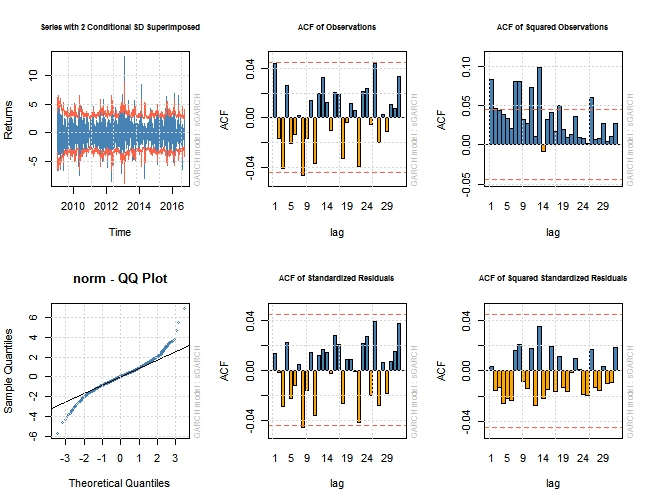
\includegraphics[width=0.9\linewidth]{figs/figevtAAPL}
	\caption[Modelo AR-GARCH de Apple Inc.]{Ajuste de APPL ao modelo AR(1)-GARCH(1,1). Autocorrelação nos quadrados das perdas e distribuição dos resíduos padronizados com caudas longas.}
	\label{fig:figevtAAPL}
\end{figure}

A tabela \ref{tab:tabevtAAPL} abaixo traz as informações sobre o modelo ajustado. Os valores estimados dos parâmetros, assim como seus erros padrões, estatística \emph{t} e valores \emph{p}. Percebe-se que de fato o modelo se ajustou aos dados, considerando que todos os parâmetros estimados são significativos com ao menos 95\% de confiança com exceção do parâmetro $\phi_1$ o qual, pelo gráfico de autocorrelação, já esperávamos fosse pouco significativo.

Ajustado este primeiro modelo, que é o equivalente a filtrar os dados originais de perda com um modelo AR-GARCH de modo que os resíduos padronizados agora sim sejam as realizações de uma variável aleatória \emph{iid}, então podemos aplicar a técnica de modelagem da cauda destes resíduos conforme a teoria de valor extremo. Cabe salientar que é fundamental fazer esta filtragem nos dados, uma vez que a POT supõe dados independentes e identicamente distribuídos, caso contrário não teríamos a convergência dada no teorema \ref{teor:pickands} de Pickands-Balkema-de Haan.

% latex table generated in R 3.3.0 by xtable 1.8-2 package
% Sun Oct 02 15:20:08 2016
\begin{table}[ht]
\centering
\caption{Par\^ametros estimados para o modelo AR-GARCH de AAPL} 
\label{tab:tabevtAAPL}
\begin{tabular}{rrrrr}
  \hline
 & Estimativa & Erro Padr\~ao & Valor t & Pr(>|t|) \\ 
  \hline
$\mu$ & -0.1683 & 0.0381 & -4.4138 & 0.0000 \\ 
  $\phi_1$ & 0.0400 & 0.0246 & 1.6282 & 0.1035 \\ 
  $\omega$ & 0.2107 & 0.0514 & 4.1011 & 0.0000 \\ 
  $\alpha_1$ & 0.0876 & 0.0187 & 4.6804 & 0.0000 \\ 
  $\beta_1$ & 0.8445 & 0.0301 & 28.0768 & 0.0000 \\ 
   \hline
\end{tabular}
\end{table}


Portanto, aplicaremos agora a modelagem POT para os resíduos padronizados, os quais sabemos não serem normalmente distribuídos e que possuem considerável curtose em excesso (vide gráfico QQ da figura \ref{fig:figevtAAPL}) e encontraremos os valores de $z_\alpha$ e $E[Z|Z>z_\alpha]$ necessários para computar os valores de $VaR_\alpha$ e $ES_\alpha$ das equações \eqref{eq:varcond} e \eqref{eq:escond}.

Os valores de $z_\alpha$ e $E[Z|Z>z_\alpha]$ foram calculados para $\alpha=0,99$ e são apresentados na tabela \ref{tab:tabevtAAPL2} abaixo juntamente com os limites  inferior e superior de seu intervalo de confiança a 95\%. Note que $E[Z|Z>z_\alpha]$ na tabela em questão foi chamado de $s_{.99}$.
% latex table generated in R 3.3.0 by xtable 1.8-2 package
% Sun Oct 02 15:17:32 2016
\begin{table}[ht]
\centering
\caption{Valores de $z_{.99}$ e $s_{.99}$ encontrados e seus
	respectivos intervalos de confian\c ca a 95\%} 
\label{tab:tabevtAAPL2}
\begin{tabular}{rrcr}
  \hline
 & Inf & Estimativa & Sup \\ 
  \hline
$z_{.99}$ & 2.40 & 2.61 & 2.89 \\ 
  $s_{.99}$ & 3.11 & 3.55 & 4.90 \\ 
   \hline
\end{tabular}
\end{table}


\begin{figure}[h]
	\centering
	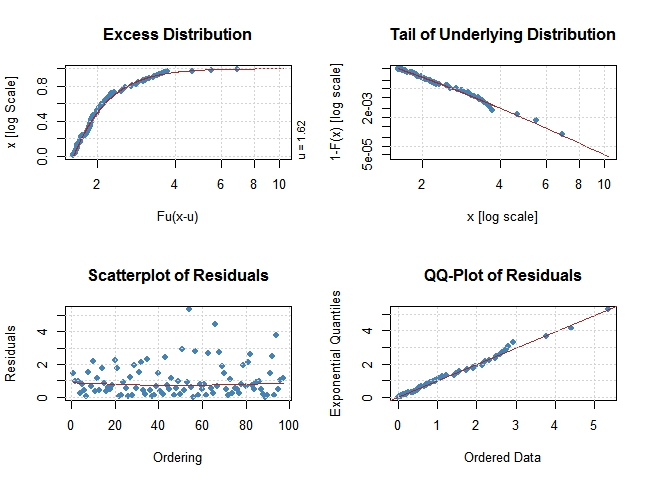
\includegraphics[width=0.9\linewidth]{figs/figevtAAPL2}
	\caption[Modelo POT de Apple Inc.]{Ajuste dos resíduos padronizados a um modelo POT. Distribuição dos excessos acima do limiar $u=1,62$.}
	\label{fig:figevtAAPL2}
\end{figure}

A figura \ref{fig:figevtAAPL2} traz algumas informações acerca do ajuste feito a uma GPD dos resíduos padronizados obtidos. Foi escolhido como limiar \emph{u} o valor de 1,62 que é o quantil de $z_t$ a 0,95. Esse valor foi ratificado através da análise qualitativa do gráfico de vida média residual (MRL plot) conforme encontrado na definição \ref{defi:meanexcess}. Com a escolha deste limiar, obtivemos 97 observações de perdas em excesso a este valor. Quantidade razoável e que nos permite calcular os parâmetros da distribuição GPD.

Pode-se verificar através da figura \ref{fig:figevtAAPL2} que os ajustes feitos foram bastante satisfatórios, principalmente com a GPD capturando muito bem a curtose em excesso na cauda da distribuição dos resíduos padronizados (\emph{tail of underlying distribution}) e os quantis dos próprios resíduos deste ajuste ficarem juntos dos valores teóricos esperados (QQ \emph{plot of residuals}).

Possuímos todos os parâmetros de nosso modelo híbrido AR-GARCH-POT para então calcularmos os valores das medidas de risco condicional dadas pelas equações \eqref{eq:varcond} e \eqref{eq:escond}. Com o modelo AR-GARCH executado no período \emph{t} obtemos as estimativas de $\mu_{t+1}$ e de $\sigma_{t+1}$ e através do modelo POT obtemos os valores de $z_\alpha$ e $E[Z|Z>z_\alpha]$, no caso do nosso exemplo escolhemos $\alpha=0,99$.

Toda esta metodologia pode ser aplicada período a período, mantendo uma memória fixa das últimas \emph{n} observações de perdas e que resultará em valores calculados para $VaR_\alpha^{t+1}$ e $ES_\alpha^{t+1}$, os quais poderão ser comparados com a realização futura de perda.

\section{Conclusão}


%\section{Processos pontuais}
%\label{sec:pp}
%
%Na seção anterior consideramos apenas a magnitude das perdas em excesso, sem nos preocuparmos com o momento da ocorrência destas. Implicitamente, consideramos que as ocorrências eram independentes entre si, uma condição necessária para a modelagem POT.
%
%Entretanto, esta suposição tipicamente é violada pelas séries financeiras, devido a autocorrelação entre retornos e principalmente ao \emph{clustering} de volatilidade nestas séries.
%
%Modelos de processos pontuais, especialmente aqueles conhecidos como processos de Hawkes, ou processos pontuais de auto-excitação, nos permitem modelar tanto as magnitudes das perdas em excesso, como a probabilidade de sua ocorrência em período futuro a depender da atual situação. Estes processos tem natureza dinâmica, assim como aquele desenvolvido na subseção anterior \ref{sec:riscocond}, e nos permitem calcular medidas condicionais de risco com a vantagem de todo o processo ser feito em apenas um único passo.
%
%A seguir apresentamos alguns conceitos teóricos sobre processos pontuais de Poisson que nos possibilitarão desenvolver o modelo de processos pontuais de auto-excitação, nos quais realmente estamos interessados. Para uma abordagem mais formal e completa sobre processos pontuais, é sugerida a leitura de \cite{Daley2003,Daley2008}.
%
%Consideremos uma sequência de variáveis aleatórias $Y_1, \ldots , Y_n$ as quais assumem valores dentro de um determinado espaço de estados $\mathcal{S}$. Dado um subconjunto $A\subset\mathcal{S}$, podemos definir a variável aleatória
%\begin{equation}
%\label{eq:pp}
%N(A)=\sum_{i=1}^{n}I_{\{Y_i\in A\}}
%\end{equation}
%que é a contagem do número de observações $Y_i$ que recaem dentro do conjunto $A$. A função $I_{\{Y_i\in A\}}$ é a chamada função indicador, sendo seu valor igual a 1 caso $Y_i$ esteja contido no subconjunto $A$ e 0 caso contrário, de forma que a soma dada pela equação \eqref{eq:pp} será justamente a contagem desejada. Neste caso diz-se que \eqref{eq:pp} define um processo pontual $N(\cdot)$. Um tipo de processo pontual de interesse é aquele de Poisson.
%
%\begin{figure}[ht]
%	\centering
%	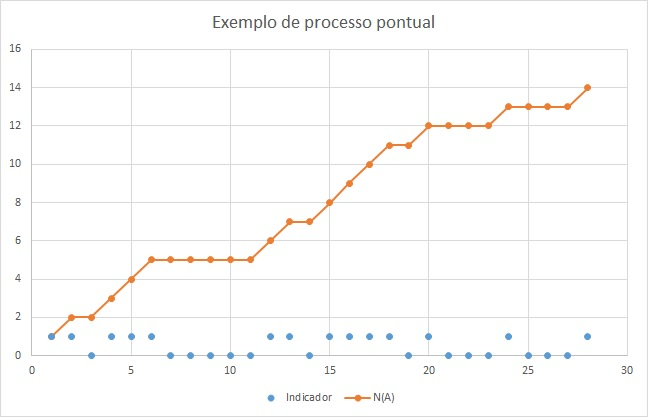
\includegraphics[width=0.9\linewidth]{figs/figevtPP}
%	\caption[Exemplo de processo pontual]{Processo pontual. Cada vez que o indicador alterna para 1 a contagem soma este valor.}
%	\label{fig:figevtpp}
%\end{figure}
%
%\begin{defi}[Processo pontual de Poisson]
%	\label{defi:poissonpp}
%	O processo pontual $N(\cdot)$ é chamado de Poisson no espaço de estados $\mathcal{S}$ e com medida de intensidade $\Lambda$ se as duas condições seguintes são satisfeitas.
%\end{defi}
%\begin{enumerate}[label=(\alph*)]
%	\item Para $A\subset\mathcal{S}$ e $k\geq 0$,
%	\begin{equation*}
%	P\left(N(A)=k\right)=
%	\begin{cases}
%	e^{-\Lambda(A)\frac{\Lambda(A)^k}{k!}}, &\Lambda(A)<\infty, \\
%	0, &\Lambda(A)=\infty .
%	\end{cases}
%	\end{equation*}
%	\item Para qualquer $m\geq 1$, se $A_1, \ldots , A_m$ são conjuntos mutuamente exclusivos de $\mathcal{S}$, então as variáveis aleatórias $N(A_1), \ldots , N(A_m)$ são independentes.
%\end{enumerate}
%
%Também deve ser definida a função intensidade (ou somente intensidade) do processo pontual, que é a derivada da medida de intensidade $\Lambda(A)$ satisfazendo a equação $\Lambda(A)=\int_A\lambda(\mathbf{x}) d\mathbf{x}$. De modo que $\lambda(\mathbf{x})$ é a função intensidade, que pela sugestão de nossa notação, pode ser uma função multivariável em um vetor $\mathbf{x}$.
%
%\begin{defi}[Processo de Poisson homogêneo]
%	\label{defi:poihomo}
%	Seja $N$ um processo de Poisson no espaço $\mathcal{S}$ com intensidade $\lambda$, então $N$ é dito homogêneo se $\lambda$ não for dependente do espaço $\mathcal{S}$, caso contrário é dito não-homogêneo.
%\end{defi}
%
%Ou seja, em um processo de Poisson homogêneo, sua intensidade depende apenas do tamanho do intervalo onde se está contando o número de ocorrências, mas não da localização deste intervalo. 
%
%Um processo de Poisson é dito \emph{marcado}, quando além dos pontos pertencentes ao subconjunto $A$, atribuímos a cada um destes pontos uma "marca"  com valor dentro do espaço $\mathcal{M}$, de forma que a série aleatória passa a ser de pares $\{(i, L_i): i\in A \text{ e } L_i \in \mathcal{M}\}$. Estas marcas podem ser entendidas como a magnitude das perdas em excesso em nosso modelo, enquanto que os pontos do processo serão os períodos em que estas perdas extraordinárias ocorrem.
%
%\begin{defi}[Processos pontuais de Poisson marcados]
%	\label{defi:pppmarcados}
%	Suponha um processo pontual de Poisson $Y(\cdot)$ em $\mathcal{S}$ com função de intensidade $\lambda$. Suponha também que, condicionalmente a $Y(\cdot)$, as marcas $\{m_i : i \in Y\}$ sejam independentes. Então $N=\{(i, m_i): i \in Y\}$ é um processo de Poisson marcado. Se as marcas são \emph{iid} com uma distribuição de probabilidades comum \emph{H}, então esta é conhecida como a distribuição das marcas.
%\end{defi}
%
%De acordo com nosso modelo de perdas extremas, podemos entendê-lo como um processo pontual de Poisson marcado ao atribuir aos eventos (i.e. perdas extremas) uma outra informação vinculada, qual seja, o valor desta perda e portanto, os pontos do processo passam a carregar a informação extra da magnitude das perdas. Assim temos um processo que mapeia pares $(i, l)$ de períodos e perdas a uma probabilidade de uma nova perda extrema.
%
%\subsection{Processos pontuais de auto-excitação}
%\label{sec:autoex}
%
%São conhecidas as evidências encontradas na literatura que os retornos de séries financeiras não são de fato \emph{iid} e portanto tampouco o são as perdas acima de um limiar. Assim, estas perdas, consideradas no tempo, não ocorrem de acordo com um processo de Poisson homogêneo, tendendo a formarem \emph{clusters} de perdas (ou retornos) extremos, que correspondem a episódios de concentração de volatilidade. Para contornar este fato, uma dentre várias possibilidades estão os processos de Hawkes, os quais fornecem uma base teórica robusta para este tipo de processos com autocorrelação.
%
%Passamos nossa atenção aos processos de Hawkes, ou processos pontuais de auto-excitação. Neste tipo de modelagem, a intensidade do processo, $\lambda(\mathbf{x})$ é dependente dos períodos e magnitudes das marcações anteriores. Traduzindo para nosso modelo de perdas acima de um limiar, a probabilidade de um novo excesso é dependente do histórico dos períodos e magnitudes dos excessos anteriores. Desta forma temos um modelo dinâmico e condicional para avaliar a probabilidade de eventos extremos, no caso em tela, de perdas excessivas.
%
%Dada a distribuição de perdas realizadas $L_1, \ldots , L_n$ e um valor de limiar \emph{u}, assumimos que existam $N_u$ excessos, cada um ocorrido em um período \emph{i}, de modo que temos a série de pares $\{(i, L_i): 1\leq i \leq n, \quad L_i > u\}$. Aqui adotamos o indexador de tempo das observações das perdas pertencente aos números naturais, logo $i\in \mathbb{N}$. Será também necessária adotar uma notação alternativa apenas para os valores das perdas que foram acima do limiar, e enumerá-las de forma consecutiva. Assim, $\{(T_j, \tilde{L}_j): j=1, \ldots , N_u\}$, com $T_j \in [1,n]$ e $\tilde{L}_j$ é o valor original da perda dado que ela esteja acima do limiar.
%
%Primeiramente consideraremos um modelo de processo pontual para os tempos das perdas em excesso somente. Façamos $Y_i=i I_{\{L_i>u\}}$, logo $Y_i$ retornará o período em que um excesso ocorreu, gerando uma lista de números naturais crescente e não repetidos. O processo pontual dos períodos destes excessos é $N(\cdot)$ no espaço $\mathcal{S}=(0, n]$, e é dado por $N(A)=\sum_{i=1}^{n}I_{\{Y_i\in A\}}$ para $A \subset \mathcal{S}$. Ou seja, nosso processo é a contagem do número de excessos ocorridos dentro de um intervalo de tempo $A$ contido em nossa amostra $\mathcal{S}$.
%
%Assumimos que este processo pontual seja do tipo Hawkes, com características de auto-excitação, portanto a intensidade em um período $i$ é condicional aos acontecimentos passados até $i$, da seguinte forma
%
%\begin{equation}
%\label{eq:condintensity}
%\lambda^*(i)=\tau + \psi \displaystyle\sum_{j:0<T_j<i}h(i-T_j, \tilde{L}_j -u)
%\end{equation}
%onde $\tau>0$, $\psi \geq 0$ e $h$ é uma função positiva, decrescente no intervalo de tempo $s=i-T_j$ e crescente na magnitude do excesso $l=\tilde{L}_j-u$. Assim, cada par ordenado de tempo e valor da perda em excesso $(T_j, \tilde{L}_j)$ anteriores ao período $t$ contribuem para a intensidade condicional do processo de Poisson. Uma conhecida parametrização para a função $h$ vem da sismologia através de \cite{Ogata1988}. Os processos pontuais de auto-excitação já vêm sendo aplicados a inferência e previsão de tremores sísmicos há décadas, e somente mais recentemente estão sendo aplicados aos "tremores"  financeiros e suas ondas de choque. O modelo proposto é chamado de \emph{Epidemic Type Aftershock Sequence} (ETAS) e adotamos a parametrização proposta em \cite{Harte2010}, abaixo:
%\begin{equation*}
%\label{eq:hsl}
%h(s, l)=e^{\delta l}\left(1+\frac{s}{\gamma}\right)^{-\rho}, \text{onde } \delta, \gamma, \rho > 0.
%\end{equation*}
%
%A função intensidade pode ser encarada como a chance instantânea de ocorrência de um ponto do processo no período $t$, \cite{Chiu2013}, portanto o fato de a transformarmos em uma função condicional resulta que temos agora uma probabilidade condicional de verificarmos no instante $t$ uma perda em excesso e por conseguinte, temos nossas medidas condicionais de risco $VaR_\alpha^t$ e $ES_\alpha^t$.
%
%Podemos então tomar nosso modelo POT de perdas acima de um determinado limiar e adequá-lo a um processo de Poisson marcado, com função intensidade auto-excitável. Pode-se separar este modelo em dois tipos, o primeiro com a distribuição das marcas do tipo \emph{iid} GPD, de forma que o valor das marcas (i.e. a magnitude das perdas em excesso) é incondicional e distribuído conforme uma distribuição genreralizada de Pareto, e um segundo tipo, onde a distribuição das próprias marcas é condicional a informação histórica, mas ainda GPD. Em \cite{ChavezDemoulin2005} existe uma implementação similar destes modelos e neste artigo alega-se a pouca evidência a favor do segundo modelo, onde os parâmetros da GPD seriam também dependentes dos pontos e marcas. Desta forma, adotamos aqui o modelo de processo de Hawkes marcado, sendo a distribuição das marcas uma distribuição do tipo GPD, dada pela equação \eqref{eq:GPD} e com a restrição adicional que $\xi>0$ de tal modo que obtemos uma distribuição com caudas longas para as perdas em excesso.
%
%Vejamos que este modelo não perde a generalização que queremos com relação ao fato de os retornos financeiros não serem \emph{iid}. Este fato está bem descrito ao adotarmos um processo de Hawkes para os pontos destes, ou seja, a dependência dos retornos é dada pela modelagem dos momentos quando estes ocorrem em excesso. A magnitude destes excessos não interferem na probabilidade de um novo evento extremo no futuro imediato. 
%
%A primeira vista esta abordagem pode parecer pouco intuitiva, mas ela está de acordo com os fatos estilizados das séries financeiras já apresentados, em especial, demonstramos que as autocorrelações entre os retornos propriamente ditos dos ativos é baixa, quando verificável. E este fato está presente em nossa abordagem quando afirmamos que a magnitude das perdas em excesso não interferem diretamente na probabilidade e na magnitude de uma nova perda extrema. As autocorrelações tipicamente encontradas nas séries financeiras são entre os retornos ao quadrado, fato que nos remete imediatamente a volatilidade. Esta sim está modelada através do processo pontual de auto-excitação, quando a função intensidade é dependente do histórico do processo até o período atual.
%
%Para encontrarmos a função densidade de probabilide (p.d.f) conjunta de nosso modelo de processo de Poisson marcado (MPP - \emph{Marked Poisson Process}) faremos uso da definição de intensidade condicional para um MPP econtrada em, \cite{Daley2003}[p. ~249] e também da p.d.f de uma GPD. Começamos pela última.
%
%A função densidade de probabilidade de uma distribuição generalizada de Pareto, parametrizada em $\xi$ e $\beta$ é dada por:
%\begin{align}
%\label{eq:pdfgpd}
%g_{\xi, \beta}(x)=\frac{1}{\beta}\left(1+\xi\frac{x}{\beta}\right)^{-1-1/\xi}, &\,\xi \neq 0
%\end{align}
%e estamos interessados nos valores de $\xi$ no intervalo $(0, 1)$.
%
%\begin{defi}[Intensidade condicional de um processo marcado de Poisson]
%	Seja N um processo regular marcado de Poisson em $\mathbb{N}\times\mathcal{M}$. A intensidade condicional de N, em relação ao seu histórico $\mathcal{H}$, é a função $\lambda^*(i, m)=\lambda^*_g(i)f^*(m|i)$.
%\end{defi}
%Onde $\lambda^*_g(i)$ é a função intensidade do processo base (i.e. dos tempos dos pontos, no nosso casso a intensidade do processo de Hawkes, dado pela equação \eqref{eq:condintensity}) e $f^*(m|i)$ é a densidade condicional das marcas no período $i$. Como estamos trabalhando com uma distribuição GPD independente dos períodos em que ocorrem as perdas extremas, $f^*(m|i)$ resume-se a nossa p.d.f de uma GPD, dada pela equação \eqref{eq:pdfgpd}.
%
%Portanto, nossa p.d.f conjunta para o modelo de processo pontual de auto-excitação das perdas acima de um limiar \emph{u}, assumindo uma função núcleo $h(s, l)=e^{\delta l}\left(1+\frac{s}{\gamma}\right)^{-\rho}$ pode ser descrita através das seguintes equações:
%\begin{align}
%g_{\xi, \beta}(x)=&\frac{1}{\beta}\left(1+\xi\frac{x-u}{\beta}\right)^{-1-1/\xi} \\
%\lambda^*_g(i)=&\tau+\psi\sum_{j:0<T_j<i}h(i-T_j, \tilde{L}_j-u) \\
%h(s, l)=&e^{\delta l}\left(1+\frac{s}{\gamma}\right)^{-\rho} \\
%s=&i-T_j, \quad l=\tilde{L}_j-u \\
%\lambda^*(i, m)=&\lambda^*_g(i)\, g_{\xi, \beta}(m) \label{eq:hawkesgpd}
%\end{align}
%
%Coletando todos os parâmetros a serem estimados no vetor $\boldsymbol{\theta}=(\tau, \psi, \delta, \gamma, \rho, \xi, \beta )$ e considerando que informamos ao modelo o valor do limiar \emph{u}, poderemos estimar todos os parâmetros do modelo através do método de estimação de máxima verossimilhança (MLE - \emph{maximum likelihood estimation}) em um único passo. A função de verossimilhança logarítimica pode ser deduzida diretamente deste conjunto de equações, sendo a equação \eqref{eq:hawkesgpd} a densidade de probabilidades de interesse para a aplicação do método.
%
%\begin{exemplo}[Processo pontual de auto-excitação da Goldman Sachs]
%	\label{exe:GS}
%	Tomaremos como exemplo a aplicação de um processo de Hawkes aos retornos da Goldman Sachs Group Inc. (\emph{ticker} GS) no período entre 05/05/1999 a 04/10/2016, compreendendo 4.384 observações.
%\end{exemplo}
%Primeiramente é necessário montar a série de pontos do processo, que nada mais são que os pares $(T_j, \tilde{L}_j-u)$, onde o valor do limiar $u$ foi escolhido como sendo o quantil $q=0,90$ de nossa amostra. Ou seja, tomamos apenas as 10\% maiores perdas de nossa amostra. A partir deste ponto, podemos fazer uma estimativa dos parâmetros do modelo através do método de maximização da verossimilhança, sendo a função de verossimilhança aquela encontrada em \cite[eq. (7) p. ~6]{Harte2010}.
%
%Uma vez obtidos os parâmetros do modelo, podemos plotar a função intensidade de base do processo de Hawkes (i. e. $\lambda^*_g(i)$) contra os períodos $i$ para verificar como esta de fato variou conforme os eventos ocorreram. Na figura \ref{fig:figevtGS} é possível verificarmos nossa estimativa da função intensidade de base e compará-la ao eventos do processo de Hawkes, ou seja, as perdas extremas verificadas.
%
%\begin{figure}[ht]
%	\centering
%	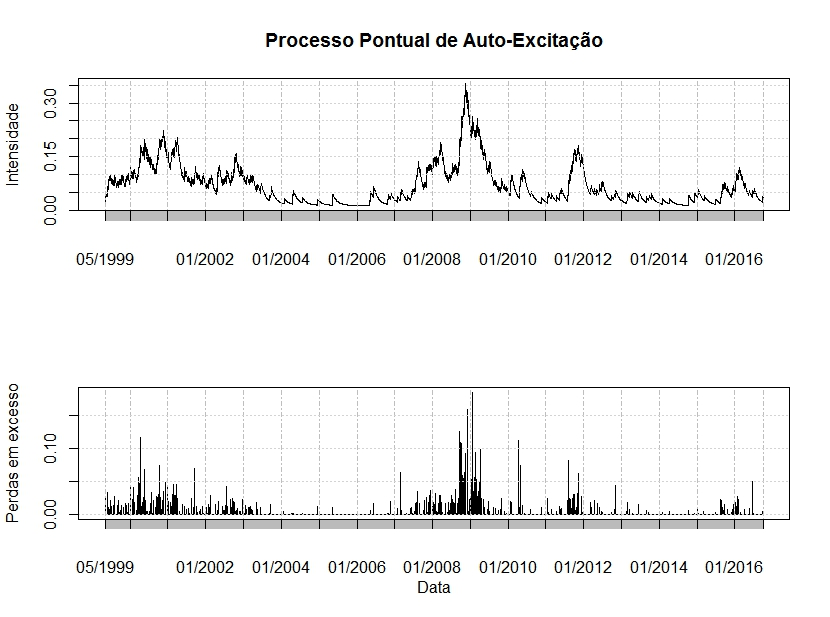
\includegraphics[width=0.9\linewidth]{figs/figevtGS}
%	\caption[Intensidade de Hawkes para Goldman Sachs]{Função intensidade de Hawkes e perdas extremas da Goldman Sachs (GS) no período entre 05/05/1999 a 04/10/2016.}
%	\label{fig:figevtGS}
%\end{figure}
%
%Podemos então calcular a probabilidade condicional de ultrapassarmos um determinado valor de perda $x$ do nosso ativo, no período $i$, dado o conjunto de informações disponíveis. Esta probabilidade nada mais é que a cauda da distribuição das perdas e portanto, o valor $1-\alpha$, onde $\alpha$ é o intervalo de confiança de nossas medidas de risco. Chamamos de $\tau^*(i+1, x)$ esta probabilidade:
%\begin{align}
%\label{eq:tau}
%\tau^*(i+1, x)=&\displaystyle\int\limits_x^\infty \lambda^*(i, y)dy \nonumber \\
%=&\lambda^*_g(i) \bar{G}_{\xi, \beta}(x-u)
%\end{align}
%
%O que esta equação nos informa é que a probabilidade de ocorrência de uma perda acima de um valor $x\geq u$ é dada pelo produto entre nossa função intensidade de base, que não depende de $x$ e a cauda da distribuição GPD das marcas do processo de Poisson. Ambas já calculadas conforme o exemplo \ref{exe:GS}. Este resultado não deve vir como uma surpresa, uma vez que a probabilidade de termos uma perda maior que um dado valor $x\geq u$, considerando o conjunto de informações até o período $i$, $\mathcal{G}_i$, sempre pode ser decomposto da seguinte forma:
%\begin{equation*}
%P(X_{i+1}>x|G_i)=P(X_{i+1}-u>x-u|X_{i+1}>u, G_i)\, P(X_{i+1}>u|G_i)
%\end{equation*}
%
%Onde primeiro termo a direita da igualdade é a cauda da distribuição das perdas em excesso, a qual supomos uma GPD independente do período $i$ e o segundo termo é a probabilidade de ocorrência de um "ponto" no processo pontual, que é justamente a função intensidade de base em um dado período $i$.
%
%Assim, a partir de $\tau^*(i+1, x)$ para encontrarmos digamos, $VaR_\alpha^{i+1}$, o que precisamos fazer é igualar $\tau^*(i+1, x)$ a $1-\alpha$ e inverter a equação para $x$. Este valor de $x$ é nossa medida de risco. Para valores de $\alpha$ suficientemente grandes, de modo que nosso quantil $VaR_\alpha^{i+1} > u$, este cálculo pode ser feito e resulta em:
%
%\begin{equation}
%\label{eq:VaRpp}
%VaR_\alpha^{i+1} = u+\frac{\beta}{\xi}\left[ \left( \frac{1-\alpha}{\lambda^*_g(i)}\right)^{-\xi}-1 \right].
%\end{equation}
%
%Veja a semelhança desta equação com aquela em \eqref{eq:VaRGPD}. Para a abordagem através de processo de Hawkes marcado, substituímos a estimação empírica não-condicional da probabilidade de acontecer um evento extremo, $\bar{F}(u)=N_u/N$ por uma estimação que acreditamos mais adequada, o processo de Hawkes na forma de sua função intensidade de base. Da mesma forma, o $ES_\alpha^{i+1}$ pode ser calculado através da equação \eqref{eq:ESGPD}.
%
%\begin{equation}
%\label{eq:ESpp}
%ES_\alpha^{i+1} = \frac{VaR_\alpha^{i+1}}{1-\xi}+\frac{\beta-\xi u}{1-\xi}
%\end{equation}
%
%Voltando ao nosso exemplo \ref{exe:GS} e aplicando as equações \eqref{eq:VaRpp} e \eqref{eq:ESpp} para a série de perdas de \emph{Goldman Sachs}, obtemos o seguinte resultado demonstrado na figura \ref{fig:figevtGS2} abaixo.
%
%\begin{figure}[h]
%	\centering
%	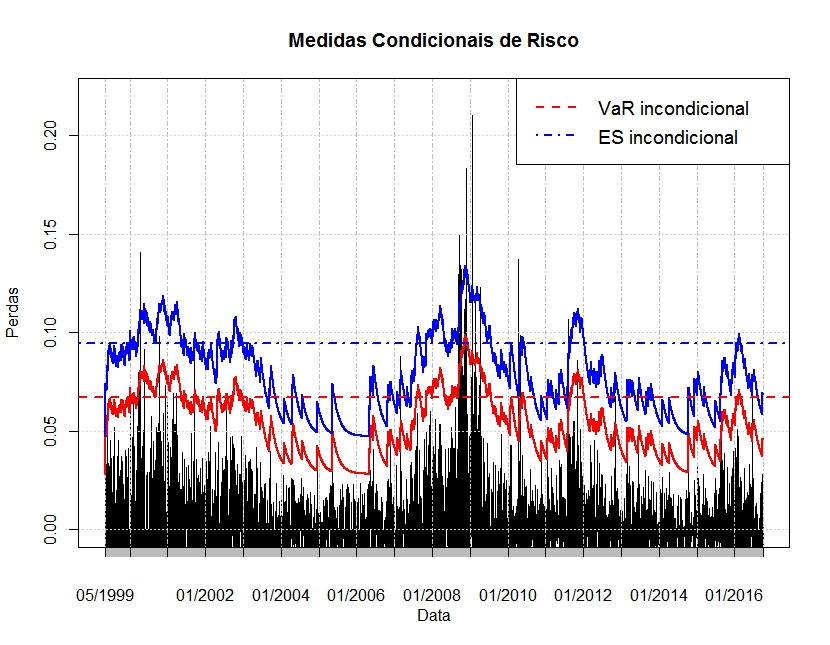
\includegraphics[width=0.9\linewidth]{figs/figevtGS2}
%	\caption[VaR e ES condicionais através de um processo pontual de auto-excitação]{VaR e ES condicionais de \emph{GS}. Linhas contínuas são as medidas condicionais, com ES sempre mais alto que o VaR. As medidas incondicionais são apresentadas para referência.}
%	\label{fig:figevtGS2}
%\end{figure}
%
%Conforme mostra a figura \ref{fig:figevtGS2}, em momentos de baixa volatilidade as medidas condicionais de risco podem cair abaixo de seus valores históricos (i.e. incondicionais) e portanto, esta abordagem pode liberar capital da instituição financeira de seus requerimentos mínimos. Por outro lado, em momentos de alta volatilidade as medidas condicionais de risco se elevam subitamente e, neste caso, a instituição deveria levantar capital rapidamente.

\section*{References}

\bibliography{library}

\end{document}
